\documentclass[a4paper]{article}

%------------------------------------------------------------
\usepackage[a4paper, total={6in, 9in}]{geometry}
\usepackage{amsmath, amssymb}
\usepackage{booktabs}
\usepackage{caption}
\usepackage{enumitem}
\usepackage{graphicx}
\usepackage{float}
\usepackage{inconsolata}
\usepackage{listings}
\usepackage{mathtools}
\usepackage{pstricks-add}
\usepackage{siunitx}
\usepackage[most]{tcolorbox}
\usepackage{tikz}
\usepackage{epstopdf} %converting to PDF
\usepackage{hyperref}

\usetikzlibrary{shapes.geometric}
\usetikzlibrary{arrows}

%------------------------------------------------------------
\graphicspath{{./fig/}}

%------------------------------------------------------------
\setlength{\parindent}{0in}

\lstdefinestyle{C++}{
	language=C++,
	basicstyle=\ttfamily,
	keywordstyle=\color{blue}\ttfamily,
	stringstyle=\color{red}\ttfamily,
	commentstyle=\color{green}\ttfamily,
	morecomment=[l][\color{magenta}]{\#},
	showstringspaces=false
}

%------------------------------------------------------------
\newtcblisting[auto counter]{sexylisting}[2][]{sharp corners, 
    fonttitle=\bfseries, colframe=gray, listing only, 
    listing options={basicstyle=\ttfamily,language=C++}, 
    title=Listing \thetcbcounter: #2, #1}

%------------------------------------------------------------
\lstset{language=C++,
        basicstyle=\ttfamily,
        keywordstyle=\color{blue}\ttfamily,
        stringstyle=\color{red}\ttfamily,
        commentstyle=\color{green}\ttfamily,
        morecomment=[l][\color{magenta}]{\#},
        showstringspaces=false
}
%------------------------------------------------------------
\tikzstyle{block} = [draw, fill=blue!20, rectangle, 
    minimum height=3em, minimum width=3em]
\tikzstyle{sum} = [draw, fill=blue!20, circle, node distance=1cm]
\tikzstyle{input} = [coordinate]
\tikzstyle{output} = [coordinate]
\tikzstyle{pinstyle} = [pin edge={to-,thin,black}]

%------------------------------------------------------------
\newlength{\arrow}
\settowidth{\arrow}{\scriptsize$1000$}
\newcommand*{\myrightarrow}[1]{\xrightarrow{\mathmakebox[\arrow]{#1}}}

%------------------------------------------------------------

\begin{document}
\title{Deep Reinforcement Learning: Robotic Arm Control}
\author{Shane Reynolds}
\maketitle

\section*{Abstract}



\section{Introduction}
Prior to 2010, state of the art speech to text was achieved by taking an audio sample input which was passed through various independently developed models, such as acoustic models, and language models, which converted the input to text. In 2010, Deep Neural Networks (DNN) started to make improvements on this approach. The DNN approach simply took the raw audio input and returned the text output, replacing the various acoustic, and language models with single network. Speech recognition with DNNs is now considered state of the art. Prior to 2012, the Computer Vision task of taking raw pixel input and labelling the picture as an output was achieved by extracting key points, using SIFT feature computation, and applying deformable part models. In 2012, ImageNet and AlexNet demonstrated performance which surpassed the current state of the art, effectively replacing the image labelling process with a single DNN. Again, prior to 2014, text-to-text machine translation was undertaken with a series of individual models and computation processes. Today, state of the art machine translation is achieved with a single DNN. The common theme in these examples is that input to output transformation, which were comprised of many individual models, been replaced by a single DNN yielding significant increases in system performance.\\

The field of robotics presents a similar story: robotic sensor input is processed, and actions in the physical world are the system output. Currently, state-of-the-art approaches to achieving this sensor input to action output transformation is done using perception models to localise the robot and map the environment, navigation models to path plan, and control models to move actuators. Thinking of a robotic system in this context presents a compelling argument for trying to replace our approach to perception, navigation, and control using a single DNN. Simple analogies aside, it must be acknowledged that robotics is more challenging than labelling an image. The main reason is that the robot's actions change the nature of the robot's environment. The implication is that we cannot collect static data to learn actions from, rather, the data set needs to be built by the robot exploring and interacting with the environment. One of the best ways that we currently know how to approach this problem is through reinforcement learning.
 
TALK ABOUT REINFORCEMENT LEARNING

This paper explores deep reinforcement learning (DRL) and its application to a three degree of freedom robotic arm. The reinforcement learning agent is trained to touch a cylindrical object which is spawned in the robot's workspace. The goal comes in two flavours: the first is to touch the cylindrical object with any part of the robot; the second, more difficult, goal is to touch the cylindrical object with the robot arm end effector. Learning takes place over repeated episodes, which are terminated when the robot successfully touches the object, or when the robot arm collides with the ground. A final reward is given when the agent reaches a terminal state. An interim rewards is assigned at each discrete time step. The interim reward function design is the main focus of the paper. The benchmark for 


\section{Background}
\subsection{Markov Decision Process}
Reinforcement Learning (RL) is a branch of machine learning that is concerned with how agents make sequential decisions to maximise some notion of a cumulative reward. Suppose that a robotic agent exists in some environment which is comprised of many discrete states, $s \in S$, such that $S$ denotes the state space. At any discrete point in time the agent can take an action $a \in A$, where $A$ denotes the action space. When the agent takes an action in a given state, the agent receives some reward, denoted with $r \in R$, where $R$ is the reward set. If an agent is in a given state, $s$, and takes and action, $a$, this will transition the agent to a new state, $s'$, and yield reward, $r$, with some given probability - these are referred to as state transition probabilities. Transition probabilities are denoted as follows:
\begin{equation}
P(S_{t+1}=s', R_{t+1}=r \ | \ S_t = s, A_t = a)
\end{equation}

The set of parameters, outlined above, make up a framework referred to as a Markov Decision Process (MDP).

\subsection{Policy}
In order for the robot to act within the environment, it needs to have a policy. A policy, $\pi$, is defined as a mapping from states to actions, that is, a rule which determines what action the robot will take for a given state. A deterministic policy, $\pi (s)$, maps a single action to a single state. A stochastic policy, $\pi (a | s)$, defines a probability distribution over the actions for a given state.

\subsection{Return}
As the robotic agent takes actions at each discrete time step, it receives a reward. The cumulative sum of this reward is referred to as the return. The return is denoted, for $N$ discrete time steps, as:
\begin{equation}
G_t = r_t + r_{1+1} + r_{t+2} + \ldots + r_{N-1}
\end{equation}

Often it is convenient to make future rewards less important that more immediate rewards. This is by multiplying each reward in the sequence by a discount factor, $\gamma \in [0,1]$. Equation (XXXX) then becomes:
\begin{equation}
G_t = r_t + \gamma r_{1+1} + \gamma^2 r_{t+2} + \ldots + \gamma^{N-1} r_{N-1} = \sum_{k = 0}^{N-1} \gamma^k r_{t+k}
\end{equation} 

\subsection{Value Function \& Action Value Function}
In order to help decide what the agent's best action to take at a particular instant it is important for the agent to know how good it is to be in a particular state. A way of measuring the ``goodness'' of a state is the \textit{value function}, $v_{\pi}(s)$, which is defined as the expected value of the return that an agent will receive while following a particular policy $\pi$ starting in some state $s$. Mathematically, this can be described as follows:
\begin{equation}
v_{\pi}(s) = \mathbb{E}_{\pi} ( G_t \ | \ s_t = s ) = \mathbb{E}_{\pi} \bigg( \sum_{k=0}^{\infty} \gamma^k r_{t+k} \ | \ s_t = s \bigg)
\end{equation}

An alternative way to express equation (XXXX) is with the Bellman equation:
\begin{equation}
v_{\pi}(s) = \sum_{a \in A(s)} \pi\big(a | s\big) \sum_{s' \in S^+, r \ \in R} P\big(S_{t+1}=s', R_{t+1} = r \ | \ S_t=s, A_t=a\big) \cdot \big(r + \gamma v_{\pi}(s')\big)
\end{equation} 

In addition to the \textit{value function}, it may be useful for the robot to measure the value of taking an action if it is in some given state - this is called an \textit{action-value function}. Formally, the \textit{action-value function}, $q_{\pi}(s,a)$, is defined as the expected value of the return that the agent will receive after taking action $a$ in state $s$, and following policy $\pi$ thereafter. Mathematically, this can be expressed as:
\begin{equation}
q_{\pi}(s,a) = \mathbb{E}_{\pi} (G_t \ | \ s_t = s, a_t = a) = \mathbb{E}_{\pi} \bigg( \sum_{k=0}^{\infty} \gamma^k r_{t+k} \ | \ S_t=s, A_t=a \bigg)
\end{equation}

\subsection{Reinforcement Learning Algorithms}
The objective of RL is to determine the policy which will maximise the expected value of the agent's cumulative reward. The value function is useful when assessing whether one policy is better than another policy. We say that some policy $\pi'$ is better than policy $\pi$ if and only if $v_{\pi'}(s) \geq v_{\pi}(s) \ \forall \ s \in S$. There is always one policy that is better than all the other policies - this policy is often referred to as the optimal policy. Whilst there may be more than one optimal policy, we denote them using $\pi^*$. They share the same \textit{value function}, denoted $v_{\pi^*}$, and are defined as:
\begin{equation}
v_{\pi^*(s)} = \max_{\pi} v_{\pi}(s), \ \forall \ s \in S
\end{equation}

Optimal policies also share the same optimal action-value functions, denoted $q_*(s,a)$, and defined as:
\begin{equation}
q_*(s,a) = \max_{\pi} q_{\pi}(s,a), \ \forall \ s \in S, \ a \in A(s)
\end{equation}

The optimal action value function, $q_*(s,a)$, is an important function because it yields the expected return for taking action $a$ in state $s$ and following the optimal policy $\pi_*$ thereafter. Determining this function allows us to derive the optimal policy. This is done by mapping each state to the action yielding the highest expected return according to $q_*$. Classical RL approaches often represent \textit{action-value} functions for low dimensional discrete problems as tables, referred to as \textit{Q-tables}. States are represented as rows and actions as columns. Each state-action pair, $(s_i, a_j)$, corresponds to an entry in the table consisting of the expected return of taking action $a_j$ from state $s_i$ and following the proposed policy. An example of this can be seen in Table XXXX which shows a toy problem consisting of three discrete states: $s_1$, $s_2$, $s_3$ and four discrete actions: $a_1$, $a_2$, $a_3$, $a_4$.\\

\begin{table}[h]
\centering
\captionof{table}{text}
\begin{tabular}{|c|c|c|c|c|}
\hline
 & $a_1$ & $a_2$ & $a_3$ & $a_4$\\
\hline
$s_1$ & -4 & 5 & \textbf{6} & 2 \\
\hline
$s_2$ & \textbf{3} & 1 & 1 & 1 \\
\hline
$s_3$ & 6 & 4 & 6 & \textbf{8} \\
\hline
$s_4$ & -6 & \textbf{4} & 3 & 3 \\
\hline
\end{tabular}
\end{table}

\vspace{0.5cm}

In this instance, suppose Table XXXX represents the optimal \textit{action-value} function, $q_*(s,a)$. The optimal policy, $\pi_*$, is therefore obtained by simply taking the actions corresponding to the bold values. Posing the RL problem this way makes it clear that the primary objective is engineering approaches which estimate $q_*(s,a)$. For problems of low dimensionality there are two main approaches: model-based methods; and model-free methods. Model-based methods try to utilise some information of the environment. Historically this was achieved by building a model of the environment from first principals and using it to learn the optimal policy or value function. The problem with starting from first principals is that if the model is not an accurate depiction of reality, then the policy learned is likely to be sub-optimal. Two popular algorithms for model based policy evaluation are Policy Iteration and Value Iteration, both described in Appendix A.\\

In contrast to model-based methods, model-free methods assume no known knowledge of the environment. Generally, these types of approaches are favoured over model-based methods since accurate environmental models are difficult to build all but the simplest of games. Model-free approaches try to learn an optimal \textit{action-value} function by exploring the world, iteratively building on the estimation, until such time that the Q-table estimation converges with $q_*(s,a)$. The optimal policy can be extracted from $q_*(s,a)$. Monte Carlo methods and Temporal Difference methods are both popular model-free approaches to solving the RL problem.

\subsubsection{Monte Carlo Methods} 
Monte Carlo (MC) methods require only a sample of episodic sequences consisting of states, actions, and rewards from an agent interacting in an environment to estimate an \textit{action-value} function for some policy $\pi$. An estimate update occurs for every visit to a \textit{state-action} pair for a given episode. A \textit{state-action} pair is said to be visited in an episode if ever the state $s$ is visited and action $a$ is taken. Once an episode is completed, the \textit{action-value} estimate for each \textit{state-action} pair is updated either using the first visit to the \textit{state-action} pair, or by averaging the returns from all visits. This process, called the \textit{evaluation} step, only represents one half of the MC implementation. Once the \textit{action-value} function for some policy $\pi$ has been estimated, MC seeks to improve on it's current policy by choosing a policy favouring actions which provide the greatest return for each state. The new policy is derived from the current Q-table estimate of $q_{\pi}(s,a)$, and this step is called the \textit{policy improvement} step. For any sub-optimal \textit{action-value} function $q$, we select the action for each $s \in S$ that provides the maximal \textit{action-value}. Mathematically, this is described as follows:
\begin{equation}
\pi(s) = \arg \max_a q(s,a)
\end{equation}

The policy evaluation and policy improvement steps are repeated iteratively, as shown in Figure XXXX. 

\begin{figure}[h]
\centering
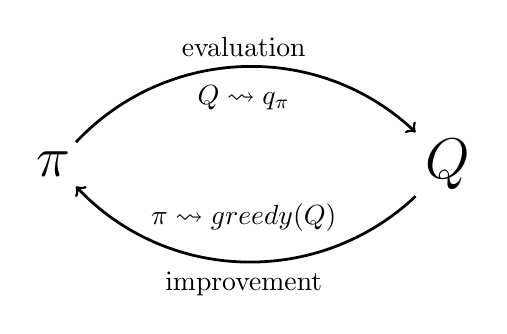
\begin{tikzpicture}
\node (A) {\huge$\pi$};
\node[right of=A, node distance=5cm] (B) {\huge$Q$};

\draw[->, line width=1pt] (A) edge[bend left=45] node[below=0.1cm] {$Q \rightsquigarrow q_\pi $} node[above] {evaluation} (B);
\draw[->, line width=1pt] (B) edge[bend left=45] node[below] {improvement} node[above=0.25cm] {$\pi \rightsquigarrow greedy(Q)$} (A);
\end{tikzpicture}
\caption{text}
\end{figure}

The MC iteration continues to repeat these two distinct steps until convergence on $q_*$ is achieved. Beginning with some arbitrary policy, $\pi_0$, this can be mathematically shown as follows:
\begin{equation*}
\pi_0 \myrightarrow{E} q_{\pi_0} \myrightarrow{I} \pi_1 \myrightarrow{E} q_{\pi_1} \myrightarrow{I} \pi_2 \myrightarrow{E} \ldots \myrightarrow{I} \pi_* \myrightarrow{E} q_*,
\end{equation*}

where $\myrightarrow{E}$ denotes a complete policy evaluation and $\myrightarrow{I}$ demotes a complete policy improvement. One of the major drawbacks with practical implementations of MC methods is that if the agent never visits a \textit{state-action} pair then the arbitrary policy initially assigned will remain in place which can lead to sub-optimal policies. For low dimensional problems, this issue is addressed by getting the agent to select random policy actions with some non-zero probability. Doing this gives the agent a curiosity type behaviour, which encourages it to explore the the state action space, as opposed to simply exploiting the current best policy. This type of behaviour is especially important when the agent first commences learning, and becomes less important as the policy estimate converges to the optimal policy.

\subsubsection{Temporal Difference Methods}


\subsection{Deep Reinforcement Learning}
For low dimensional problems Monte Carlo methods or Temporal Difference methods work fine, however, as the dimensionality of the problem grows it becomes more difficult to successfully build a discrete representation of the the optimal q function - requires more iterations and takes a larger amount of compute.

to get around this problem, we can used neural networks
\subsubsection{Experience Replay}
\subsubsection{Fixed Q-Targets}

\newpage

\section{Robotic Arm Reinforcement Learning Problem}
Newborn babies are typically unable to coordinate their arms to reliably grasp objects within their reach, however, as early as 4 months old babies can locate and pick up large objects such as blocks. One simple way to think about the baby developing this skill is to envision the baby taking repeated attempts to locate and pick up an object - if the baby successfully grasps the object then it feels happy, if it is unable to grasp the object then it feels sad. Simplifying things further we might crudely imagine the baby as a system comprised of an arm full of sensors which can detect object collisions, and a camera allowing vision of it's own arm interacting in the environment. This is the problem that this paper attempts to simulate and solve using DRL. The robotic arm is simulated in Gazebo, and consists of three revolute joints providing three degrees of freedom. A cylindrical object is placed within the work space of the robot, and the robot can observe the both its arm and the environment with an external camera. The scene set up is shown in Figure XXXX.
\begin{figure}[h]
\centering
\frame{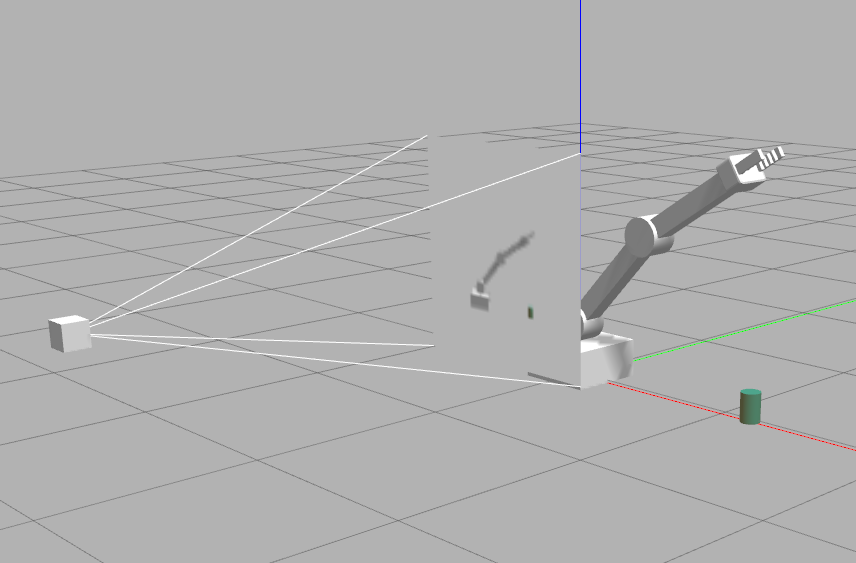
\includegraphics[scale=0.4]{arm_image_2}}
\caption{Robotic arm with three revolute joints: one in the base; a shoulder joint; and an elbow joint. The robot is tasked with touching the green cylindrical object, and can see itself interacting in the environment.}
\end{figure}

The task is simple - the robotic arm must reach towards and touch the object. The robot can view itself and the object with a camera, and the it knows what it's joint angles are. A single attempt at touching the object is called an episode, and can consist of many actions. At each discrete time step during an episode, the robot can take a discrete action for a single one of its three joints. The robot can move a joint position by a small amount, or change the joint velocity by a small amount. After each action, the robot receives an interim reward. An episode terminates when the robot collides with the ground; or successfully touches the object; or XXXX seconds elapse for a given episode. Upon episode termination, the robot receives a final reward. Commencing a new episode re-initialises the joint angles so that the robot arm stretches upwards, and the object is repositioned back in front of the robot.\\

Initialisation of the DQN agent, which contains the neural network being trained, requires a call to the \texttt{dqnAgent::Create()} function shown in Listing 1. The function takes a number of hyperparameters which are important for specifying the neural network architecture. Some of the more important parameters include the type of numerical optimiser to use, the learning rate for the network, batch size, and whether to use Long Short Term Memory (LSTM).

\begin{figure}[h]\scriptsize
\begin{sexylisting}{DQN Initialisation}
agent = dqnAgent::Create(INPUT_WIDTH, INPUT_HEIGHT, INPUT_CHANNELS, DOF*2,
			 OPTIMIZER, LEARNING_RATE, REPLAY_MEMORY, BATCH_SIZE, 
		  	 GAMMA, EPS_START, EPS_END, EPS_DECAY, 
		  	 USE_LSTM, LSTM_SIZE, ALLOW_RANDOM, DEBUG_DQN);
\end{sexylisting}
\end{figure}

\newpage

There were two choices when designing the action space: allow an action to change a joint position; or allow an action to change a joint velocity. Changing the joint position directly was problematic since instantaneously altering joint positions by a small amount at each time step, led to  jittery robotic movements. Further it is obviously impossible to move joints instantaneously in the real world. Actions were instead defined to be the change of the angular velocity for a given joint, which yielded much smoother looking robotic movements. The robot action implementation was developed as part of a method for the DQN agent called \texttt{ArmPlugin::updateAgent()}

\begin{figure}[h]\scriptsize
\begin{sexylisting}{listing}
float velocity = 0.0; // TODO - Set joint velocity based on whether action is even or odd.

if (action % 2 == 0){
    velocity = vel[action/2] + actionVelDelta;
}else{
    velocity = vel[action/2] - actionVelDelta;
}


if( velocity < VELOCITY_MIN )
    velocity = VELOCITY_MIN;

if( velocity > VELOCITY_MAX )
    velocity = VELOCITY_MAX;

vel[action/2] = velocity;
\end{sexylisting}
\end{figure}

WHAT IS THE ARCHITECTURE OF THE NEURAL NETWORK THAT IS BEING USED TO DELIVER THE DRL\\


\section{Collisions}
Two different types of collisions were monitored at each time step. The first type of collision is bad, and occurs if any part of the arm collides with the ground. This was implemented as part of the \texttt{ArmPlugin::OnUpdate()} method. WHAT DOES THE PIECE OF CODE DO? The implementation code snippet can be seen in Listing XXXX.
\begin{figure}[h]\scriptsize
\begin{sexylisting}
cconst math::Box& gripBBox = gripper->GetBoundingBox();
const float groundContact = 0.05f;

if (gripBBox.min.z < groundContact){
						
    if(DEBUG){printf("GROUND CONTACT, EOE\n");}
    printf("Robot hit ground");
    rewardHistory = REWARD_LOSS;
    newReward     = true;
    endEpisode    = true;
}
\end{sexylisting}
\end{figure}

The second type of collision represents a successful episode, and is triggered according to to different criteria. First criteria is when any part of the robot touches the object. The second criteria is when the robot end effector touches the object. The code snippet was implemented as part of the XXXX method. TALK ABOUT WHAT IT WAS DESIGNED TO DO. The implementation can be seen in Listing XXXX.
\begin{figure}[h]\scriptsize
\begin{sexylisting}{listingxxx}
for (unsigned int i = 0; i < contacts->contact_size(); ++i){
	
    if( strcmp(contacts->contact(i).collision2().c_str(), COLLISION_FILTER) == 0 )
        continue;
		
    if (strcmp(contacts->contact(i).collision1().c_str(), COLLISION_ITEM) == 0 ||
        strcmp(contacts->contact(i).collision2().c_str(), COLLISION_ITEM) == 0){
			
            std::cout << "Collision between[" << contacts->contact(i).collision1()
                      << "] and [" << contacts->contact(i).collision2() << "]\n";

            rewardHistory = REWARD_WIN;

            newReward  = true;
            endEpisode = true;

            return;
	}
}
\end{sexylisting}
\end{figure} 


\section{Reward Function}
Rewards are given to the agent when ever an episode terminates. If the agent experiences a collision with the ground, or if the episode times out, the agent is deemed to have failed the task and is given a punitive reward of XXXX. If the agent is successful in touching the object, then it is successful in its task and is given a reward of XXXX to promote the behaviour. In addition to final rewards, the agent also receives interim rewards at each time step. Just like the final rewards, the agent can be given a positive reward if the behaviour over the time step is desirable, or a negative reward if the behaviour is undesirable.

TALK MORE ABOUT THE REWARD FUNCTIONS THAT COULD BE DEPLOYED.

\begin{figure}[h]\scriptsize
\begin{sexylisting}{listing}
if (gripBBox.min.z >= groundContact){
    
    // compute the reward from distance to the goal
    const float distGoal = BoxDistance(gripBBox, propBBox); 

    if( episodeFrames > 1 ){
        
        // compute the change in distance to the goal
        const float distDelta  = lastGoalDistance - distGoal;

        // compute the smoothed moving average of the delta of the distance to the goal
        avgGoalDelta  = (avgGoalDelta * 0.5) + (distDelta * (1.0 - 0.5));
        rewardHistory = avgGoalDelta;
        newReward     = true;
    }
    
    lastGoalDistance = distGoal;
    
}
\end{sexylisting}
\end{figure}



\section{Hyperparameters}
TALK ABOUT THE SELECTION OF INPUT WIDTH AND INPUT HEIGHT, TALK ABOUT THE CHOICE OF OPTIMISER, TALK ABOUT THE CHOICE OF LEARNING RATE, TALK ABOUT THE CHOICE OF REPLAY MEMORY, TALK ABOUT THE CHOICE OF BATCH SIZE, TALK ABOUT THE CHOICE OF USING LSTM, TALK ABOUT THE CHOICE OF THE LSTM SIZE

\begin{figure}[h]\scriptsize
\begin{sexylisting}{listing}

// define hyperparameters 
#define INPUT_WIDTH   64
#define INPUT_HEIGHT  64
#define OPTIMIZER "RMSprop"
#define LEARNING_RATE 0.01f
#define REPLAY_MEMORY 10000
#define BATCH_SIZE 8
#define USE_LSTM false
#define LSTM_SIZE 32

\end{sexylisting}
\end{figure}


\section{Results}
TALK ABOUT HOW LONG IT TOOK FOR THE ROBOT TO REACH THE DESIRED SOLUTION SPACE FOR EACH OF THE TASKS\\

INCLUDE SCREENSHOTS AND VARIOUS VIDEOS OF EACH OF THE 


\section{Discussion}
TALK ABOUT THE FACT THAT THE SUCCESS OF THE REINFORCEMENT LEARNING TASK LARGELY COMES DOWN TO THE DETERMINATION OF A REWARD FUNCTION THAT ALLOWS THE ROBOT TO CONVERGE ON THE DESIRED BEHAVIOUR.

\section{Future Work}
TALK ABOUT THE FACT THAT THERE ARE ADDITIONAL CAMERAS AND THAT THE OBJECT COULD BE RANDOMLY PLACED THROUGHOUT THE ENVIRONMENT AND THAT ROBOT BASE COULD BE MOVED ALSO TO TRY TO GET THE ROBOT TO LEARN MORE EXOTIC POLICIES

\bibliography{my_bib}
\bibliographystyle{ieeetr}

\end{document}